% vim: set foldmethod=marker foldlevel=0:

\documentclass[a4paper]{article}
\usepackage[UKenglish]{babel}

% NOTE: hyperref has to come before preamble
\usepackage{hyperref}

\usepackage{preamble}

\usepackage{graphicx}
\graphicspath{ {./imgs/} }

\fancyhead[L]{MA144 Assignment 4}
\title{MA144 Methods of Mathematical Modelling 2, Assignment 4}

\begin{document}

\maketitle

\setlength{\parindent}{0em}
\setlength{\parskip}{1em}

% {{{ Q1
\question{1}

Let $C$ be the curve parametrised by \begin{align*}
x(\theta) &= (1-r) \cos \theta + r \cos \l( \f{1-r}{r} \theta \r) \\[1ex]
y(\theta) &= (1-r) \sin \theta - r \sin \l( \f{1-r}{r} \theta \r)
\end{align*}
where $r = \df1k$ and $k \in \N$.
Therefore $C$ is also parametrised by \begin{align*}
x(\theta) &= \l( 1 - \f1k \r) \cos \theta + \f1k \cos \l( (k-1) \theta \r) \\[1ex]
y(\theta) &= \l( 1 - \f1k \r) \sin \theta - \f1k \sin \l( (k-1) \theta \r)
\end{align*}

Also let $D$ be the area enclosed by $C$. We want the area of $D$, which is $\ds \iint_D \d x \d y$. Green's Theorem states that $$\iint_D \l( \pdd Qx - \pdd Py \r) \d x \d y = \oint_C \l( P \d x + Q \d y \r)$$

So if we just choose $P$ and $Q$ such that $\ds \pdd Qx - \pdd Py = 1$, then we can apply Green's Theorem to simplify the double integral to a single integral. We will choose $Q(x, y) = x$ and $P(x, y) = 0$.

Therefore the area is \begin{align*}
\oint_C x \d y &= \oint_C x(\theta) \dd y\theta \d \theta\\[1ex]
&= \int_0^{2\pi} \l(
	\f{k-1}k \cos \theta + \f1k \cos ((k-1) \theta) \r)
	\\ &\qquad \times \l(
		\f{k-1}k \cos \theta
		- \f{k-1}k \cos ((k-1) \theta)
	\r) \d \theta\\[1ex]
%
&= \int_0^{2\pi} \bigg(
	\f{(k-1)^2}{k^2} \cos^2 \theta
	- \f{(k-1)^2}{k^2} \cos \theta \cos ((k-1) \theta)
	\\ &\qquad + \f{k-1}{k^2} \cos \theta \cos ((k-1) \theta)
	- \f{k-1}{k^2} \cos^2 ((k-1) \theta)
\bigg) \d \theta\\[1ex]
%
&= \f{k-1}{k^2} \int_0^{2\pi} \Big(
	(k-1) \cos^2 \theta
	+ (2-k) \cos \theta \cos ((k-1) \theta)
	\\ &\qquad - \cos^2 ((k-1) \theta)
\Big) \d \theta\\[1ex]
%
&= \f{k-1}{2k^2} \int_0^{2\pi} \Big(
	(k-1) (\cos 2\theta + 1)
	+ 2(2-k) \cos \theta \cos ((k-1) \theta)
	\\ &\qquad - \cos (2(k-1) \theta + 1)
\Big) \d \theta\\[1ex]
%
&= \f{k-1}{2k^2} \l[
	\f{k-1}2 \sin 2\theta
	- \f1{2k-2} \sin ((2k-2) \theta)
	+ (k-2) \theta
\r]_0^{2\pi}
	\\ &\qquad + \f{k-1}{2k^2} \int_0^{2\pi}
		2(2-k) \cos \theta \cos ((k-1) \theta)
	\d \theta\\[1ex]
%
&= \f{k-1}{2k^2} (k-2) 2\pi
	\\ &\qquad + \f{k-1}{2k^2} \int_0^{2\pi} \l(
		\cos \l( (k-1) \theta + \theta \r) + \cos \l( (k-1) \theta - \theta \r)
	\r) \d \theta\\[1ex]
%
&= \f{\pi (k-1) (k-2)}{k^2}
	+ \f{k-1}{2k^2} \int_0^{2\pi} \l(
		\cos k \theta + \cos \l( (k-2) \theta \r)
	\r) \d \theta\\[1ex]
%
&= \f{\pi (k-1) (k-2)}{k^2}
	+ \f{k-1}{2k^2} \l[ \f1k \sin k \theta + \f1{k-2} \sin ((k-2) \theta) \r]_0^{2\pi}\\[1ex]
%
&= \f{\pi (k-1) (k-2)}{k^2}
\end{align*}

% The correct answer as given by \href{https://www.sagemath.org/}{SageMath} is \begin{align*}
% &\phantom{=}\ \ \pi - \f{3\pi}k + \f{2\pi}{k^2}\\[1ex] % From symbolic SageMath
% &= \f{\pi (k^2 - 3k + 2)}{k^2}\\[1ex]
% &= \f{\pi (k-1) (k-2)}{k^2} % From observation of specific results from SageMath
% \end{align*}

See also \href{https://www.desmos.com/calculator/lt9gbsamu1}{this Desmos graph} that I made while doing this question.

% }}}

% {{{ Q2
\newquestion{2}

Let $\ul F(x, y, z) = \begin{pmatrix} y^2 \\ x \\ z \end{pmatrix}$ and let $S$ be the surface parametrised by $$\ul r(u,v) = \begin{pmatrix} u \cos v \\ u \sin v \\ 3 - u \sin v \end{pmatrix}$$
where $u \in [0,1]$ and $v \in [0, 2\pi]$.

\subsection{~}

It is fairly simple to notice by inspection that $\ul r(u, v)$ parametrises the section of the plane $z = 3-y$ where $x^2 + y^2 \le 1$. Therefore the outward-pointing unit normal is in this case upward-pointing, so it will be the branch with positive $z$ component.

First, we need the curl of $\ul F$: $$\nabla \times \ul F = \begin{pmatrix} \partial_x \\ \partial_y \\ \partial_z \end{pmatrix} \times \begin{pmatrix} y^2 \\ x \\ z \end{pmatrix} = \begin{pmatrix} 0 \\ -0 \\ 1 - 2y \end{pmatrix}$$

To find the normal vector, we also need the partial derivatives of $\ul r$: $$\ul r_u(u, v) = \begin{pmatrix} \cos v \\ \sin v \\ - \sin v \end{pmatrix} \qquad \ul r_v(u, v) = \begin{pmatrix} -u \sin v \\ u \cos v \\ u \cos v \end{pmatrix}$$

Then we get \begin{align*}
\ul{\hat n} \d S &= \pm (\ul r_u \times \ul r_v) \d u \d v\\[1ex]
&= \pm \begin{pmatrix} 2u \sin v \cos v \\ -(u \cos^2 v - u \sin^2 v) \\ u \cos^2 v + u \sin^2 v \end{pmatrix} \d u \d v\\[1ex]
&= \pm \begin{pmatrix} 2u \sin v \cos v \\ -u \cos 2v \\ u \end{pmatrix} \d u \d v
\end{align*}
We want the $z$ component to be positive as discussed earlier, so we choose the positive branch.

Therefore \begin{align*}
\iint_S \nabla \times \ul F \cdot \ul{\hat n} \d S &= \iint_S \begin{pmatrix} 0 \\ 0 \\ 1 - 2u \sin v \end{pmatrix} \cdot \begin{pmatrix} 2u \sin v \cos v \\ -u \cos 2v \\ u \end{pmatrix} \d u \d v\\[1ex]
&= \iint_S (u - 2 u^2 \sin v) \d u \d v\\[1ex]
&= \intlim 0{2\pi} {\intlim 01 {(u - 2 u^2 \sin v)} u} v\\[1ex]
&= \intlim 0{2\pi} {\l[ \f12 u^2 - \f23 u^3 \sin v \r]_{u=0}^1} v\\[1ex]
&= \intlim 0{2\pi} {\l( \f12 - \f23 \sin v \r)} v\\[1ex]
&= \l[ \f12 v + \f23 \cos v \r]_0^{2\pi}\\[1ex]
&= \pi + \f23 - \f23\\
&= \pi
\end{align*}

\subsection{~}

Stokes' Theorem states the integral we found in part~\textbf{(a)} is equal to $\ds \oint_C \ul F \cdot \d \ul r$ where $C$ is the boundary curve of $S$.

The geometry of $S$ is very simple, so it's clear that $C$ is just the level set where $u=1$. Therefore we can parametrise $C$ as $$\ul r(t) = \begin{pmatrix} \cos t \\ \sin t \\ 3 - \sin t \end{pmatrix}$$

Then we get $$\dd {\ul r}t = \begin{pmatrix} -\sin t \\ \cos t \\ \cos t \end{pmatrix}$$

And so, \begin{align*}
\oint_C \ul F \cdot \d \ul r &= \oint_C \ul F \cdot \dd {\ul r}t \d t\\[1ex]
&= \intlim 0{2\pi} {\begin{pmatrix} y^2 \\ x \\ z \end{pmatrix} \cdot \begin{pmatrix} -\sin t \\ \cos t \\ \cos t \end{pmatrix}} t\\[1ex]
&= \intlim 0{2\pi} {\begin{pmatrix} \sin^2 t \\ \cos t \\ 3 - \sin t \end{pmatrix} \cdot \begin{pmatrix} -\sin t \\ \cos t \\ \cos t \end{pmatrix}} t\\[1ex]
&= \intlim 0{2\pi} {(-\sin^3 t + \cos^2 t + 3 \cos t - \sin t \cos t)} t\\[1ex]
&= \intlim 0{2\pi} {\l( -\sin t (1 - \cos^2 t) + \f12 (\cos 2 t + 1) + 3 \cos t - \sin t \cos t \r)} t\\[1ex]
&= \intlim 0{2\pi} {\l( -\sin t + \sin t \cos^2 t + \f12 \cos 2 t + \f12 + 3 \cos t - \sin t \cos t \r)} t\\[1ex]
&= \l[ \cos t - \f13 \cos^3 t + \f14 \sin 2t + \f t2 + 3 \sin t - \f12 \sin^2 t \r]_0^{2\pi}\\[1ex]
&= 1 - \f13 + \pi - \l( 1 - \f13 \r)\\[1ex]
&= \pi
\end{align*}
This matches the integral from part~\textbf{(a)}, so Stokes' Theorem holds in this situation.

% }}}

% {{{ Q3
\newquestion{3}

$$\ul r(u, v) = \begin{pmatrix} (2 + \cos u) \cos v \\ (2 + \cos u) \sin v \\ \sin u \end{pmatrix} \qquad u, v \in [0, 2\pi]$$

\subsection{~}

\begin{figure}[h]
	\centering
	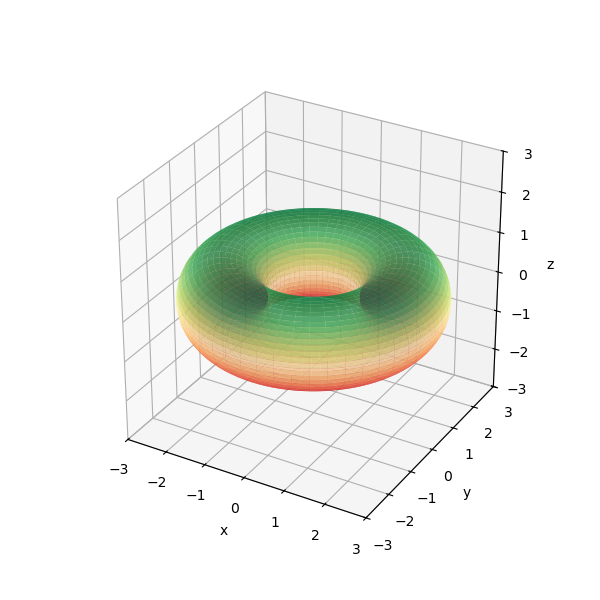
\includegraphics[scale=0.8]{Q3a-torus}
	\caption{A torus, plotted with matplotlib in Python}
	\label{fig:torus-plot}
\end{figure}

\begin{figure}[h]
	\centering
	
\includegraphics[scale=0.35]{Q3a-code}
	% TODO: Add proper GitHub link
	\caption{The code used to generate the plot in Figure~\ref{fig:torus-plot}. The code can also be found \href{https://github.com/DoctorDalek1963/uni}{on GitHub}}
\end{figure}

\clearpage
\subsection{~}

Let $\ul F(x, y, z) = (x, 0, 0)$, so $\nabla \cdot \ul F = 1$. By the Divergence Theorem, $$\iiint_V \nabla \cdot \ul F \d V = \iint_S \ul F \cdot \ul{\hat n} \d S$$
Therefore the volume of the torus is $\ds \iint_S \ul F \cdot \ul{\hat n} \d S$.

To find the normal vector, we want the partial derivatives of $\ul r$: $$
\ul r_u = \begin{pmatrix} -\sin u \cos v \\ -\sin u \sin v \\ \cos u \end{pmatrix} \qquad
\ul r_v = \begin{pmatrix} -(2 + \cos u) \sin v \\ (2 + \cos u) \cos v \\ 0 \end{pmatrix}
$$
Then we cross them and get \begin{align*}
\ul r_u \times \ul r_v &= \begin{pmatrix} -(2 + \cos u) \cos v \cos u \\ -(2 + \cos u) \sin v \cos u \\ -(2 + \cos u) \cos^2 v \sin u - (2 + \cos u) \sin^2 v \sin u \end{pmatrix}\\[1ex]
&= \begin{pmatrix} -(2 + \cos u) \cos v \cos u \\ -(2 + \cos u) \sin v \cos u \\ -(2 + \cos u) \sin u \end{pmatrix}
\end{align*}

Just by thinking about the geometry of the parametrisation, we can see that as $u$ increases, a point moves around the small circle anti-clockwise (in the poloidal direction) and as $v$ increases, a point moves around the big circle anti-clockwise (in the toroidal direction).

Therefore, by the right hand rule, $\ul r_u \times \ul r_v$ will point inwards, so we want the negative version.

Therefore \begin{align*}
\iiint_V \d V &= \iiint_V \nabla \cdot \ul F \d V\\[1ex]
&= \iint_S \ul F \cdot \ul{\hat n} \d S\\[1ex]
&= \iint_S \ul F \cdot \f{-(\ul r_u \times \ul r_v)}{\| \ul r_u \times \ul r_v \|} \| \ul r_u \times \ul r_v \| \d u \d v \\[1ex]
&= \iint_S \ul F \cdot (-(\ul r_u \times \ul r_v)) \d u \d v \\[1ex]
&= \iint_S \begin{pmatrix} (2 + \cos u) \cos v \\ 0 \\ 0 \end{pmatrix} \cdot \begin{pmatrix} (2 + \cos u) \cos v \cos u \\ (2 + \cos u) \sin v \cos u \\ (2 + \cos u) \sin u \end{pmatrix} \d u \d v \\[1ex]
&= \iint_S (2 + \cos u)^2 \cos^2 v \cos u \d u \d v \\[1ex]
&= \intlim 0{2\pi} {\intlim 0{2\pi} {\cos^2 v (4 \cos u + 4 \cos^2 u + \cos^3 u)} u} v\\[1ex]
&= \intlim 0{2\pi} {\cos^2 v} v \intlim 0{2\pi} {(4 \cos u + 4 \cos^2 u + \cos^3 u)} u\\[1ex]
&= \f12 \intlim 0{2\pi} {(\cos 2v + 1)} v \intlim 0{2\pi} {(4 \cos u + 2 \cos 2u + 2 + \cos u (1 - \sin^2 u))} u\\[1ex]
&= \f12 \l[ \f12 \sin 2v + v \r]_0^{2\pi} \intlim 0{2\pi} {(2 + 5 \cos u + 2 \cos 2u - \cos u \sin^2 u)} u\\[1ex]
&= \f12 \l( 2 \pi \r) \l[ 2u + 5 \sin u + \sin 2u + \f13 \sin^3 u \r]_0^{2\pi}\\
&= \pi \l( 4\pi \r)\\
&= 4 \pi^2
\end{align*}

The torus in the question appears to have major radius $R=2$ and minor radius $r=1$, so my volume calculation matches the expected volume of $2\pi^2 R r^2 = 4\pi^2$ in this case.

% }}}

\end{document}
